%!TEX TS-program = xelatex
%!TEX encoding = UTF-8 Unicode
% Awesome CV LaTeX Template for CV/Resume
%
% This template has been downloaded from:
% https://github.com/posquit0/Awesome-CV
%
% Author:
% Claud D. Park <posquit0.bj@gmail.com>
% http://www.posquit0.com
%
% Template license:
% CC BY-SA 4.0 (https://creativecommons.org/licenses/by-sa/4.0/)
%


%-------------------------------------------------------------------------------
% CONFIGURATIONS
%-------------------------------------------------------------------------------
% A4 paper size by default, use 'letterpaper' for US letter
\documentclass[11pt, a4paper]{awesome-cv}

% Configure page margins with geometry
\geometry{left=1.4cm, top=.8cm, right=1.4cm, bottom=1.8cm, footskip=.5cm}

% Specify the location of the included fonts
\fontdir[fonts/]

% Color for highlights
% Awesome Colors: awesome-emerald, awesome-skyblue, awesome-red, awesome-pink, awesome-orange
%                 awesome-nephritis, awesome-concrete, awesome-darknight
\colorlet{awesome}{awesome-skyblue}
% Uncomment if you would like to specify your own color
% \definecolor{awesome}{HTML}{CA63A8}

% Colors for text
% Uncomment if you would like to specify your own color
% \definecolor{darktext}{HTML}{414141}
% \definecolor{text}{HTML}{333333}
% \definecolor{graytext}{HTML}{5D5D5D}
% \definecolor{lighttext}{HTML}{999999}

% Set false if you don't want to highlight section with awesome color
\setbool{acvSectionColorHighlight}{true}

% If you would like to change the social information separator from a pipe (|) to something else
\renewcommand{\acvHeaderSocialSep}{\quad\textbar\quad}
\usepackage{pdfpages}

%-------------------------------------------------------------------------------
%	PERSONAL INFORMATION
%	Comment any of the lines below if they are not required
%-------------------------------------------------------------------------------
% Available options: circle|rectangle,edge/noedge,left/right
\photo{./cv/profile.jpg}
\name{Albert H.}{van Zyl}
\position{Electrical Engineer: \\ Expected Graduation November 2022 \\ Age: 22} %{\enskip\cdotp\enskip}Security Expert}
\address{17 Somerset Street, Somerset West, 7130 , Cape Town, Western Cape, South Africa}

\mobile{(+27) 82-087-5058}
\email{albertvzsmail@gmail.com}
%\homepage{www.posquit0.com}
\github{AlbertEE00}
\linkedin{albert-van-zyl-b357101b9}
% \gitlab{gitlab-id}
% \stackoverflow{SO-id}{SO-name}
% \twitter{@twit}
% \skype{skype-id}
% \reddit{reddit-id}
% \medium{madium-id}
% \googlescholar{googlescholar-id}{name-to-display}
%% \firstname and \lastname will be used
% \googlescholar{googlescholar-id}{}
% \extrainfo{extra informations}

\quote{"If I have seen further it is by standing on the shoulders of Giants." \\ -Isaac Newton}

%-------------------------------------------------------------------------------
\begin{document}

% Print the header with above personal informations
% Give optional argument to change alignment(C: center, L: left, R: right)
\makecvheader

% Print the footer with 3 arguments(<left>, <center>, <right>)
% Leave any of these blank if they are not needed
\makecvfooter
  {\today}
  {Albert H. van Zyl~~~·~~~Curriculum Vitae}
  {\thepage}


%-------------------------------------------------------------------------------
%	CV/RESUME CONTENT
%	Each section is imported separately, open each file in turn to modify content
%-------------------------------------------------------------------------------
%-------------------------------------------------------------------------------
%	SECTION TITLE
%-------------------------------------------------------------------------------
\cvsection{Summary}


%-------------------------------------------------------------------------------
%	CONTENT
%-------------------------------------------------------------------------------
I am a passionate and hard working Electrical and Electronic Engineering, with an interest in the fields of Engineering, Science and Technology. I am extremely interested in all aspects of electronics, including: computers,  robotics, smart-phones, micro-electronics, and IC and PCB manufacturing. I studied at Stellenbosch University, completing my degree BEng Electronic and Electrical Engineering (2019-2022) with an average of 73\% and receiving 21 distinctions. I am currently employed full time at Rheinmetall Denel Munition for my second year of employment as a Junior Electronic Engineer in the Product Development Departedment, envolved in the development of 40mm grenades, Fuzes and SAD's for munitions.


%-------------------------------------------------------------------------------
%	SECTION TITLE
%-------------------------------------------------------------------------------
\cvsection{Education}


%-------------------------------------------------------------------------------
%	CONTENT
%-------------------------------------------------------------------------------
\begin{cventries}

%---------------------------------------------------------
  \cventry
    {BEng in Electrical and Electronic, 4 years} % Degree
    {University of Stellenbosch} % Institution
    {Stellenbosch, South Africa} % Location
    {2019-2022} % Date(s)
    {
      \begin{cvitems} % Description(s) bullet points
        \item {Golden Key Award through 2019-2022 (top 20\% in degree)}
        \item {73\% degree average up to date}
        \item {21 distinctions up to date}
      \end{cvitems}
    }
  \cventry
{National Senior Certificate ${\enskip\cdotp\enskip}$ 7 distinctions} % Degree
{Boland Agricultural School } % Institution
{Paarl, South Africa} % Location
{2014-2018} % Date(s)
{
	  \begin{cvitems} % Description(s) bullet points
	  	\item {7$^{th}$ in Western Cape for Physical Science}
	  	\item {1$^{st}$ in South Africa for Agricultural Technology}
	  	\item {91\% matric average }
	  \end{cvitems}
}

%---------------------------------------------------------
\end{cventries}

%-------------------------------------------------------------------------------
%	SECTION TITLE
%-------------------------------------------------------------------------------
\cvsection{Skills}


%-------------------------------------------------------------------------------
%	CONTENT
%-------------------------------------------------------------------------------
\begin{cvskills}

%---------------------------------------------------------
%  \cvskill
%    {DevOps} % Category
%    {AWS, Docker, Kubernetes, Rancher, Vagrant, Packer, Terraform, Jenkins, CircleCI} % Skills

%---------------------------------------------------------
%  \cvskill
%    {Back-end} % Category
%    {Koa, Express, Django, REST API} % Skills
%
%%---------------------------------------------------------
%  \cvskill
%    {Front-end} % Category
%    {Hugo, Redux, React, HTML5, LESS, SASS} % Skills

%---------------------------------------------------------
  \cvskill
    {Programming} % Category
    {Python, JAVA, C, C++, Assembly (ARM), VHDL, Embed Programming, Matlab, Spice, LaTeX, PLC (ladder-logic)} % Skills

%---------------------------------------------------------
\cvskill
{Electronic Engineering} % Category
{Digital \& Analogue Circuit Design} % Skills


%---------------------------------------------------------
  \cvskill
    {Languages} % Category
    {English, Afrikaans} % Skills
    
%---------------------------------------------------------


\end{cvskills}

%-------------------------------------------------------------------------------
%	SECTION TITLE
%-------------------------------------------------------------------------------
\cvsection{Experience}


%-------------------------------------------------------------------------------
%	CONTENT
%-------------------------------------------------------------------------------
\begin{cventries}

%---------------------------------------------------------
  \cventry
{Vacation Work: IC Testing and Characterization Team} % Job title
{Azoteq} % Organization
{Paarl, South Africa} % Location
{2022 (5 weeks)} % Date(s)
{
	\begin{cvitems} % Description(s) of tasks/responsibilities
		\item {Worked alongside IC Engineers on designing a custom testing station for their IP}
		\item {Worked on the analysis of manufactured IC wafer's data and wrote Python software to utilize HDF5 formats over csv to optimize data analysis.}
	\end{cvitems}
}

%---------------------------------------------------------

  \cventry
    {Vacation Work: PLC Programming and System Design} % Job title
    {Gossamer Packaging Machinery} % Organization
    {Somerset West,Western Cape, South Africa} % Location
    {2021 (4 weeks)} % Date(s)
    {
      \begin{cvitems} % Description(s) of tasks/responsibilities
        \item {Worked alongside the companies main programmer (PLC-Programmer) to program and design a conveyor system to transport fruit produce in boxes throughout a factory.}
      \end{cvitems}
    }

%---------------------------------------------------------

%  \cventry
%    {Researcher} % Job title
%    {Undergraduate Research, Machine Learning Lab(Prof. Seungjin Choi)} % Organization
%    {Pohang, S.Korea} % Location
%    {Mar. 2016 - Exp. Jun. 2017} % Date(s)
%    {
%      \begin{cvitems} % Description(s) of tasks/responsibilities
%        \item {Researched classification algorithms(SVM, CNN) to improve accuracy of human exercise recognition with wearable device.}
%        \item {Developed two TIZEN applications to collect sample data set and to recognize user exercise on SAMSUNG Gear S.}
%      \end{cvitems}
%    }
%
%%---------------------------------------------------------
%  \cventry
%    {Software Engineer \& Security Researcher (Compulsory Military Service)} % Job title
%    {R.O.K Cyber Command, MND} % Organization
%    {Seoul, S.Korea} % Location
%    {Aug. 2014 - Apr. 2016} % Date(s)
%    {
%      \begin{cvitems} % Description(s) of tasks/responsibilities
%        \item {Lead engineer on agent-less backtracking system that can discover client device's fingerprint(including public and private IP) independently of the Proxy, VPN and NAT.}
%        \item {Implemented a distributed web stress test tool with high anonymity.}
%        \item {Implemented a military cooperation system which is web based real time messenger in Scala on Lift.}
%      \end{cvitems}
%    }
%
%%---------------------------------------------------------
%  \cventry
%    {Game Developer Intern at Global Internship Program} % Job title
%    {NEXON} % Organization
%    {Seoul, S.Korea \& LA, U.S.A} % Location
%    {Jan. 2013 - Feb. 2013} % Date(s)
%    {
%      \begin{cvitems} % Description(s) of tasks/responsibilities
%        \item {Developed in Cocos2d-x an action puzzle game(Dragon Buster) targeting U.S. market.}
%        \item {Implemented API server which is communicating with game client and In-App Store, along with two other team members who wrote the game logic and designed game graphics.}
%        \item {Won the 2nd prize in final evaluation.}
%      \end{cvitems}
%    }
%
%%---------------------------------------------------------
%  \cventry
%    {Researcher for <Detecting video’s torrents using image similarity algorithms>} % Job title
%    {Undergraduate Research, Computer Vision Lab(Prof. Bohyung Han)} % Organization
%    {Pohang, S.Korea} % Location
%    {Sep. 2012 - Feb. 2013} % Date(s)
%    {
%      \begin{cvitems} % Description(s) of tasks/responsibilities
%        \item {Researched means of retrieving a corresponding video based on image contents using image similarity algorithm.}
%        \item {Implemented prototype that users can obtain torrent magnet links of corresponding video relevant to an image on web site.}
%      \end{cvitems}
%    }
%
%%---------------------------------------------------------
%  \cventry
%    {Software Engineer Trainee} % Job title
%    {Software Maestro (funded by Korea Ministry of Knowledge and Economy)} % Organization
%    {Seoul, S.Korea} % Location
%    {Jul. 2012 - Jun. 2013} % Date(s)
%    {
%      \begin{cvitems} % Description(s) of tasks/responsibilities
%        \item {Performed research memory management strategies of OS and implemented in Python an interactive simulator for Linux kernel memory management.}
%      \end{cvitems}
%    }
%
%%---------------------------------------------------------
%  \cventry
%    {Software Engineer} % Job title
%    {ShitOne Corp.} % Organization
%    {Seoul, S.Korea} % Location
%    {Dec. 2011 - Feb. 2012} % Date(s)
%    {
%      \begin{cvitems} % Description(s) of tasks/responsibilities
%        \item {Developed a proxy drive smartphone application which connects proxy driver and customer. Implemented overall Android application logic and wrote API server for community service, along with lead engineer who designed bidding protocol on raw socket and implemented API server for bidding.}
%      \end{cvitems}
%    }
%
%%---------------------------------------------------------
%  \cventry
%    {Freelance Penetration Tester} % Job title
%    {SAMSUNG Electronics} % Organization
%    {S.Korea} % Location
%    {Sep. 2013, Mar. 2011 - Oct. 2011} % Date(s)
%    {
%      \begin{cvitems} % Description(s) of tasks/responsibilities
%        \item {Conducted penetration testing on SAMSUNG KNOX, which is solution for enterprise mobile security.}
%        \item {Conducted penetration testing on SAMSUNG Smart TV.}
%      \end{cvitems}
%      %\begin{cvsubentries}
%      %  \cvsubentry{}{KNOX(Solution for Enterprise Mobile Security) Penetration Testing}{Sep. 2013}{}
%      %  \cvsubentry{}{Smart TV Penetration Testing}{Mar. 2011 - Oct. 2011}{}
%      %\end{cvsubentries}
%    }

%---------------------------------------------------------
\end{cventries}

%%-------------------------------------------------------------------------------
%	SECTION TITLE
%-------------------------------------------------------------------------------
\cvsection{Extracurricular Activity}


%-------------------------------------------------------------------------------
%	CONTENT
%-------------------------------------------------------------------------------
\begin{cventries}

%---------------------------------------------------------
  \cventry
    {Core Member} % Affiliation/role
    {B10S (B1t 0n the Security, Underground hacker team)} % Organization/group
    {S.Korea} % Location
    {Nov. 2011 - PRESENT} % Date(s)
    {
      \begin{cvitems} % Description(s) of experience/contributions/knowledge
        \item {Gained expertise in penetration testing areas, especially targeted on web application and software.}
        \item {Participated on a lot of hacking competition and won a good award.}
        \item {Held several hacking competitions non-profit, just for fun.}
      \end{cvitems}
    }

%---------------------------------------------------------
  \cventry
    {Member} % Affiliation/role
    {WiseGuys (Hacking \& Security research group)} % Organization/group
    {S.Korea} % Location
    {Jun. 2012 - PRESENT} % Date(s)
    {
      \begin{cvitems} % Description(s) of experience/contributions/knowledge
        \item {Gained expertise in hardware hacking areas from penetration testing on several devices including wireless router, smartphone, CCTV and set-top box.}
        \item {Trained wannabe hacker about hacking technique from basic to advanced and ethics for white hackers by hosting annual Hacking Camp.}
      \end{cvitems}
    }

%---------------------------------------------------------
  \cventry
    {Core Member \& President at 2013} % Affiliation/role
    {PoApper (Developers' Network of POSTECH)} % Organization/group
    {Pohang, S.Korea} % Location
    {Jun. 2010 - Jun. 2017} % Date(s)
    {
      \begin{cvitems} % Description(s) of experience/contributions/knowledge
        \item {Reformed the society focusing on software engineering and building network on and off campus.}
        \item {Proposed various marketing and network activities to raise awareness.}
      \end{cvitems}
    }

%---------------------------------------------------------
  \cventry
    {Member} % Affiliation/role
    {PLUS (Laboratory for UNIX Security in POSTECH)} % Organization/group
    {Pohang, S.Korea} % Location
    {Sep. 2010 - Oct. 2011} % Date(s)
    {
      \begin{cvitems} % Description(s) of experience/contributions/knowledge
        \item {Gained expertise in hacking \& security areas, especially about internal of operating system based on UNIX and several exploit techniques.}
        \item {Participated on several hacking competition and won a good award.}
        \item {Conducted periodic security checks on overall IT system as a member of POSTECH CERT.}
        \item {Conducted penetration testing commissioned by national agency and corporation.}
      \end{cvitems}
    }

%---------------------------------------------------------
  \cventry
    {Member} % Affiliation/role
    {MSSA (Management Strategy Club of POSTECH)} % Organization/group
    {Pohang, S.Korea} % Location
    {Sep. 2013 - Jun. 2017} % Date(s)
    {
      \begin{cvitems} % Description(s) of experience/contributions/knowledge
        \item {Gained knowledge about several business field like Management, Strategy, Financial and marketing from group study.}
        \item {Gained expertise in business strategy areas and inisght for various industry from weekly industry analysis session.}
      \end{cvitems}
    }

%---------------------------------------------------------
\end{cventries}

%%-------------------------------------------------------------------------------
%	SECTION TITLE
%-------------------------------------------------------------------------------
\cvsection{Honors \& Awards}


%-------------------------------------------------------------------------------
%	SUBSECTION TITLE
%-------------------------------------------------------------------------------
\cvsubsection{International}


%-------------------------------------------------------------------------------
%	CONTENT
%-------------------------------------------------------------------------------
\begin{cvhonors}

%---------------------------------------------------------
  \cvhonor
    {Finalist} % Award
    {DEFCON 26th CTF Hacking Competition World Final} % Event
    {Las Vegas, U.S.A} % Location
    {2018} % Date(s)

%---------------------------------------------------------
  \cvhonor
    {Finalist} % Award
    {DEFCON 25th CTF Hacking Competition World Final} % Event
    {Las Vegas, U.S.A} % Location
    {2017} % Date(s)

%---------------------------------------------------------
  \cvhonor
    {Finalist} % Award
    {DEFCON 22nd CTF Hacking Competition World Final} % Event
    {Las Vegas, U.S.A} % Location
    {2014} % Date(s)

%---------------------------------------------------------
  \cvhonor
    {Finalist} % Award
    {DEFCON 21st CTF Hacking Competition World Final} % Event
    {Las Vegas, U.S.A} % Location
    {2013} % Date(s)

%---------------------------------------------------------
  \cvhonor
    {Finalist} % Award
    {DEFCON 19th CTF Hacking Competition World Final} % Event
    {Las Vegas, U.S.A} % Location
    {2011} % Date(s)

%---------------------------------------------------------
  \cvhonor
    {6th Place} % Award
    {SECUINSIDE Hacking Competition World Final} % Event
    {Seoul, S.Korea} % Location
    {2012} % Date(s)

%---------------------------------------------------------
\end{cvhonors}


%-------------------------------------------------------------------------------
%	SUBSECTION TITLE
%-------------------------------------------------------------------------------
\cvsubsection{Domestic}


%-------------------------------------------------------------------------------
%	CONTENT
%-------------------------------------------------------------------------------
\begin{cvhonors}

%---------------------------------------------------------
  \cvhonor
    {3rd Place} % Award
    {WITHCON Hacking Competition Final} % Event
    {Seoul, S.Korea} % Location
    {2015} % Date(s)

%---------------------------------------------------------
  \cvhonor
    {Silver Prize} % Award
    {KISA HDCON Hacking Competition Final} % Event
    {Seoul, S.Korea} % Location
    {2017} % Date(s)

%---------------------------------------------------------
  \cvhonor
    {Silver Prize} % Award
    {KISA HDCON Hacking Competition Final} % Event
    {Seoul, S.Korea} % Location
    {2013} % Date(s)

%---------------------------------------------------------
  \cvhonor
    {2nd Award} % Award
    {HUST Hacking Festival} % Event
    {S.Korea} % Location
    {2013} % Date(s)

%---------------------------------------------------------
  \cvhonor
    {3rd Award} % Award
    {HUST Hacking Festival} % Event
    {S.Korea} % Location
    {2010} % Date(s)

%---------------------------------------------------------
  \cvhonor
    {3rd Award} % Award
    {Holyshield 3rd Hacking Festival} % Event
    {S.Korea} % Location
    {2012} % Date(s)

%---------------------------------------------------------
  \cvhonor
    {2nd Award} % Award
    {Holyshield 3rd Hacking Festival} % Event
    {S.Korea} % Location
    {2011} % Date(s)

%---------------------------------------------------------
  \cvhonor
    {5th Place} % Award
    {PADOCON Hacking Competition Final} % Event
    {Seoul, S.Korea} % Location
    {2011} % Date(s)

%---------------------------------------------------------
\end{cvhonors}

%%-------------------------------------------------------------------------------
%	SECTION TITLE
%-------------------------------------------------------------------------------
\cvsection{Presentation}


%-------------------------------------------------------------------------------
%	CONTENT
%-------------------------------------------------------------------------------
\begin{cventries}

%---------------------------------------------------------
  \cventry
    {Presenter for <Hosting Web Application for Free utilizing GitHub, Netlify and CloudFlare>} % Role
    {DevFest Seoul by Google Developer Group Korea} % Event
    {Seoul, S.Korea} % Location
    {Nov. 2017} % Date(s)
    {
      \begin{cvitems} % Description(s)
        \item {Introduced the history of web technology and the JAM stack which is for the modern web application development.}
        \item {Introduced how to freely host the web application with high performance utilizing global CDN services.}
      \end{cvitems}
    }

%---------------------------------------------------------
  \cventry
    {Presenter for <DEFCON 20th : The way to go to Las Vegas>} % Role
    {6th CodeEngn (Reverse Engineering Conference)} % Event
    {Seoul, S.Korea} % Location
    {Jul. 2012} % Date(s)
    {
      \begin{cvitems} % Description(s)
        \item {Introduced CTF(Capture the Flag) hacking competition and advanced techniques and strategy for CTF}
      \end{cvitems}
    }

%---------------------------------------------------------
  \cventry
    {Presenter for <Metasploit 101>} % Role
    {6th Hacking Camp - S.Korea} % Event
    {S.Korea} % Location
    {Sep. 2012} % Date(s)
    {
      \begin{cvitems} % Description(s)
        \item {Introduced basic procedure for penetration testing and how to use Metasploit}
      \end{cvitems}
    }

%---------------------------------------------------------
\end{cventries}

\newpage
%-------------------------------------------------------------------------------
%	SECTION TITLE
%-------------------------------------------------------------------------------
\cvsection{Writing}


%-------------------------------------------------------------------------------
%	CONTENT
%-------------------------------------------------------------------------------
\begin{cventries}
	
%---------------------------------------------------------
  \cventry
    {Undergraduate Student} % Role
    {Thesis: Weather Station with E-Paper Display} % Title
    {Stellenbosch University} % Location
    {2022} % Date(s)
    {
      \begin{cvitems} % Description(s)
        \item {Writing up of thesis, full description of design, implementation and testing of a desk mounted Weather Station with a focus on low power operation using an ESP32 and E-Paper Display}
      \end{cvitems}
    }

%---------------------------------------------------------
  \cventry
    {Undergraduate Student} % Role
    {Report for E-Design 314 \& 344} % Title
    {Stellenbosch University} % Location
    {2021} % Date(s)
    {
      \begin{cvitems} % Description(s)
        \item {Writing up of report, full description of design, implementation and testing of a 8x8 LED matrix Game pad, using STM32 Micro-controller, button inputs and a variable voltage slider}
        \item {Writing up of report, full description of design, implementation and testing of a solar and battery powered auto switching flash light, with full analogue design of power circuitry (and battery charging), analogue logic design and parameter measuring and displaying through a Python program}
      \end{cvitems}
    }

%---------------------------------------------------------
\end{cventries}

%%-------------------------------------------------------------------------------
%	SECTION TITLE
%-------------------------------------------------------------------------------
\cvsection{Program Committees}


%-------------------------------------------------------------------------------
%	CONTENT
%-------------------------------------------------------------------------------
\begin{cvhonors}

%---------------------------------------------------------
  \cvhonor
    {Problem Writer} % Position
    {2016 CODEGATE Hacking Competition World Final} % Committee
    {S.Korea} % Location
    {2016} % Date(s)

%---------------------------------------------------------
  \cvhonor
    {Organizer \& Co-director} % Position
    {1st POSTECH Hackathon} % Committee
    {S.Korea} % Location
    {2013} % Date(s)

%---------------------------------------------------------
  \cvhonor
    {Staff} % Position
    {7th Hacking Camp} % Committee
    {S.Korea} % Location
    {2012} % Date(s)

%---------------------------------------------------------
  \cvhonor
    {Problem Writer} % Position
    {1st Hoseo University Teenager Hacking Competition} % Committee
    {S.Korea} % Location
    {2012} % Date(s)

%---------------------------------------------------------
  \cvhonor
    {Staff \& Problem Writer} % Position
    {JFF(Just for Fun) Hacking Competition} % Committee
    {S.Korea} % Location
    {2012} % Date(s)

%---------------------------------------------------------
\end{cvhonors}



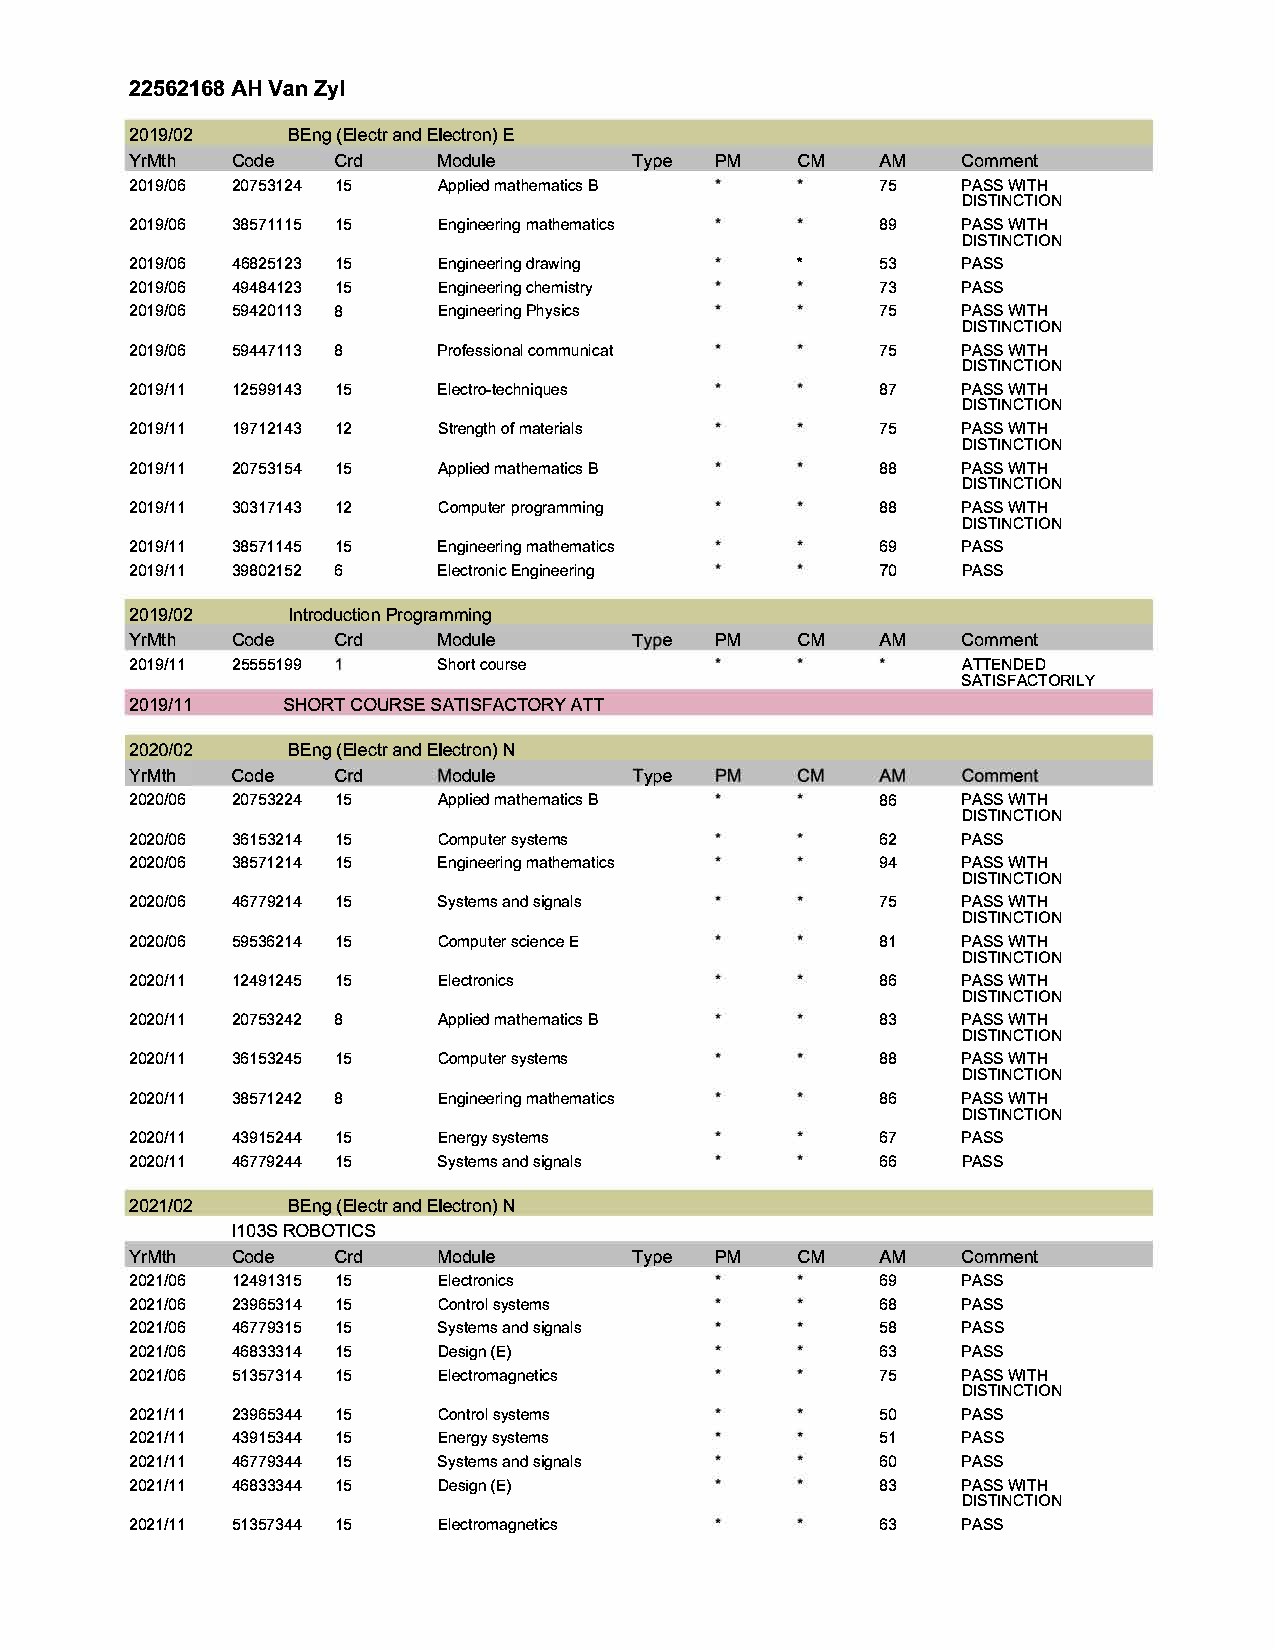
\includepdf[pages=-]{cv/AcademicHist22562168.pdf}
\includepdf[pages=-]{cv/MC.pdf}
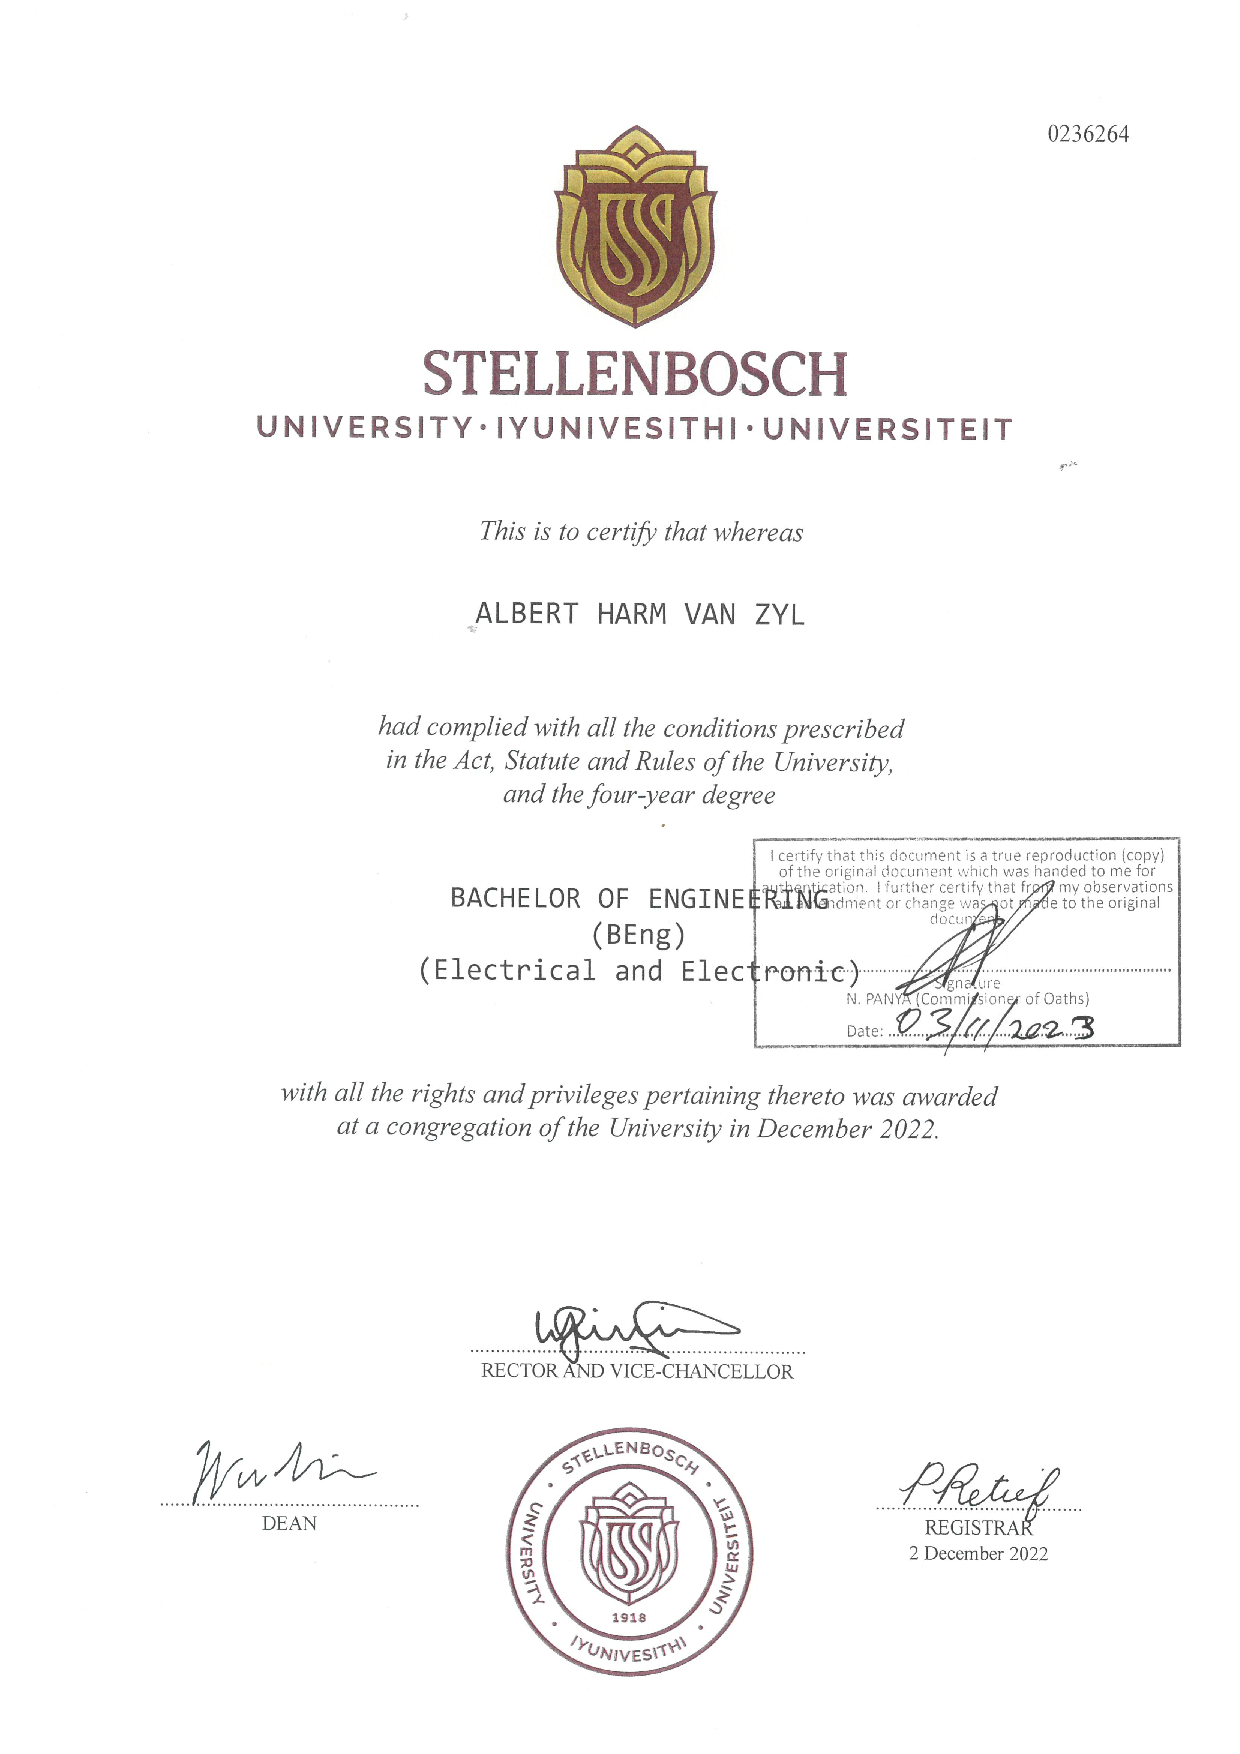
\includepdf[pages=-]{cv/Qualification.pdf}

\includepdf[pages=-]{cv/Altium-Essentials-Certificate-Albert-Van-Zyl.pdf}

%-------------------------------------------------------------------------------
\end{document}
